\documentclass[ppt2.tex]{subfiles}

%\usepackage{pgfplots}
%\pgfplotsset{width=4cm,compat=newest}
\begin{document}
\pgfplotsset{compat=1.8,width=4cm,compat=newest}
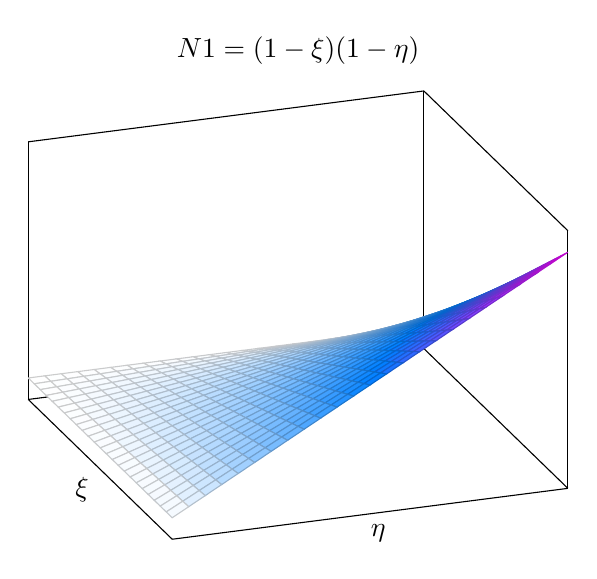
\begin{tikzpicture}
  \begin{axis}[colormap/cool,
  title = {$N1=(1-\xi)(1-\eta)$},
  ticks=none,
  %axis x line*=box,axis y line*=box, 
  %axis z line=none, 
  				view/h=70,	
  				%,hide axis
  				%axis on top,
				%axis lines*=box, 
				  	 ,xlabel = $\xi$
     , ylabel = $\eta$, 				
  				]
    \addplot3[surf,
	domain=-1:1,
	domain y=-1:1,    
    ] {0.25*(1 + x + y + x*y)};
  \end{axis}
\end{tikzpicture}
~
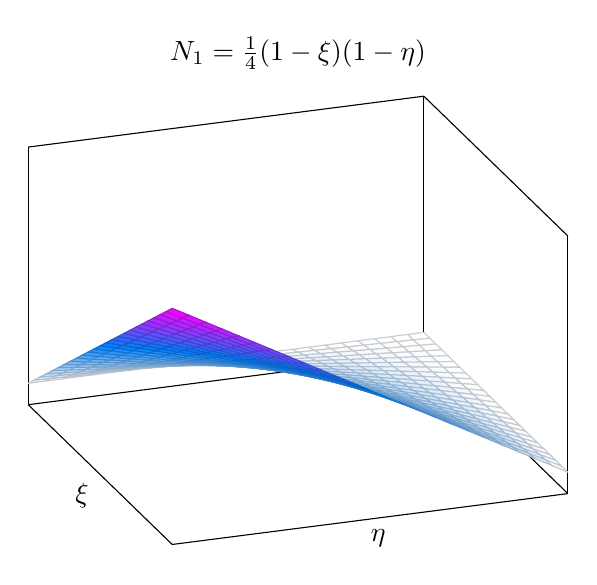
\begin{tikzpicture}
  \begin{axis}[colormap/cool,
  	%hide axis,
  	view/h=70,
  	ticks=none,
  	title = { $N_1=\frac{1}{4}(1-\xi)(1-\eta)$ },
  	 xlabel = $\xi$
     , ylabel = $\eta$,
     axis lines*=box, 
  	]
    \addplot3[surf,
	domain=-1:1,
	domain y=-1:1,    
    ]  {0.25*(1 + x - y - x*y)};
  \end{axis}
 
  
\end{tikzpicture}

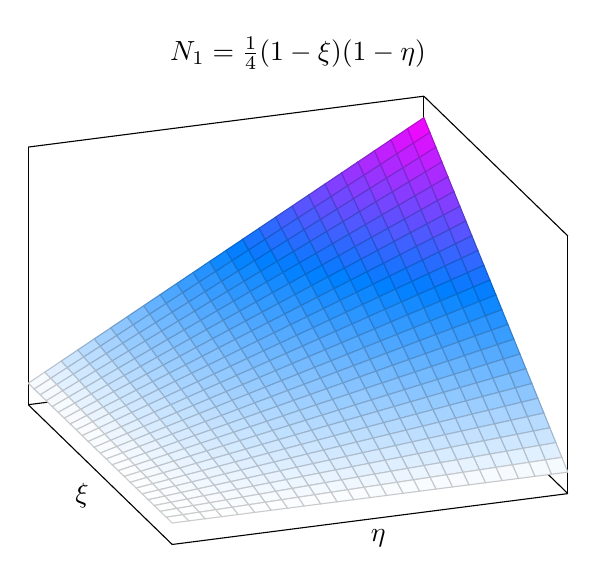
\begin{tikzpicture}
  \begin{axis}[colormap/cool,
  %,hide axis
  view/h=70,
  ticks=none,
  title = { $N_1=\frac{1}{4}(1-\xi)(1-\eta)$ },
    	 xlabel = $\xi$
     , ylabel = $\eta$
  ,axis lines*=box,
   ]
    \addplot3[surf,
	domain=-1:1,
	domain y=-1:1,    
    ]  {0.25*(1 - x + y - x*y)};
  \end{axis}
\end{tikzpicture}
~
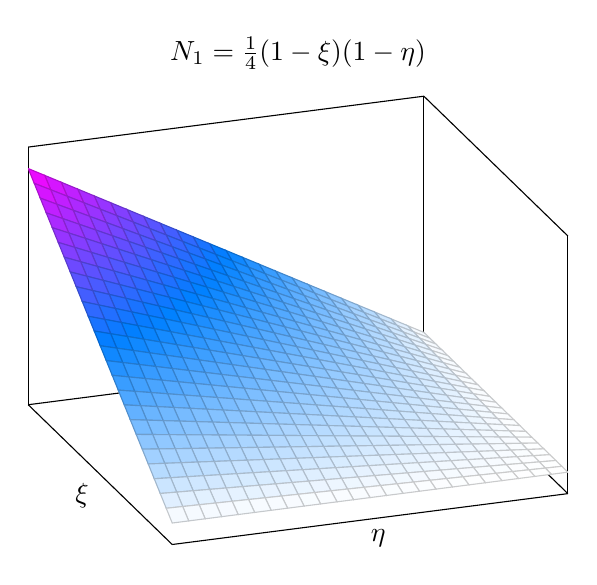
\begin{tikzpicture}
  \begin{axis}[colormap/cool,
  %,hide axis,
  view/h=70,
  ticks=none,
  title = { $N_1=\frac{1}{4}(1-\xi)(1-\eta)$ },
    	 xlabel = $\xi$
     , ylabel = $\eta$
    ,axis lines*=box,
  ]
    \addplot3[surf,
	domain=-1:1,
	domain y=-1:1,    
    ]  {0.25*(1 - x - y + x*y)};
  \end{axis}
\end{tikzpicture}






\end{document}